%% This is based on the leaflet.tex file present in the texlive-leaflet module
%% 
%% Copyright 2014 Ankur Sinha for the Fedora Marketing Team - marketing@lists.fedoraproject.org
% Please e-mail the marketing team if you have any questions with this document

\def\filename{fedora-flyer-workstation.tex}
\documentclass[
%%notumble,
%%nofoldmark,
%%dvipdfm,
%%portrait,
%%titlepage,
%%nocombine,
%%a3paper,
%%debug,
%%nospecialtricks,
%%draft,
10pt
]{leaflet}


%\renewcommand*\foldmarkrule{.3mm}
%\renewcommand*\foldmarklength{5mm}

\usepackage[T1]{fontenc}
\usepackage{textcomp}
% Use this to change the paper format
\usepackage{fancyhdr}
\usepackage{graphicx}

%%\usepackage[default]{cantarell} %% Use option ``defaultsans'' to use cantarell as sans serif only
%%\usepackage[default]{comfortaa} %% looks better
%%\usepackage[T1]{fontenc}

%% helvetica
\usepackage{helvet}
\renewcommand*{\familydefault}{\sfdefault}

\usepackage[dvipsnames,usenames]{color}
\definecolor{FedoraBlue}{cmyk}{1,0.46,0,0}
\definecolor{ResolutionBlue}{cmyk}{0.573,.462,0,0.541}
\definecolor{LIGHTGRAY}{gray}{.9}
\usepackage[colorlinks=true,urlcolor=FedoraBlue]{hyperref}

%%\setlength\footskip{2cm}

\newcommand*\defaultmarker{\textsuperscript\textasteriskcentered}

%%\title{Fedora workstation}
\title{
\includegraphics[keepaspectratio,width=0.8\textwidth]{Logo_fedoralogo.png}\vspace{1cm}\\
\includegraphics[keepaspectratio,scale=0.5]{workstation_logo_only.png}\\\vspace{0.5cm}\LARGE{\textcolor{ResolutionBlue}{WORKSTATION\\\vspace{0.2cm}21}}}
\date{\Large{\textcolor{FedoraBlue}{\href{http://fedoraproject.org}{http://fedoraproject.org}}}}
\author{\href{mailto:marketing@lists.fedoraproject.org}{marketing@lists.fedoraproject.org}}

\CutLine*{1}% Dotted line without scissors
%%\CutLine{6}%  Dotted line with scissors
\CutLine*{6}%  Dotted line with scissors

%% Use better logo for the workstation
%%\AddToBackground{1}{%  Background of a small page
%%  \put(20,530){
\includegraphics{workstation-logo.png}}}

%\AddToBackground{5}{%  Background of a small page
%  \put(0,0){\textcolor{Cerulean}{\rule{\paperwidth}{\paperheight}}}}

\AddToBackground*{2}{% Background of a large page
  \put(\LenToUnit{.5\paperwidth},\LenToUnit{.5\paperheight}){%
    \makebox(0,0)[c]{%
      \resizebox{.9\paperwidth}{!}{\rotatebox{35.26}{%
        \textsf{\textbf{\textcolor{LIGHTGRAY}{DRAFT}}}}}}}}

\begin{document}

\maketitle
\thispagestyle{empty}
\vspace{5cm}
\begin{center}\small{Fedora and the Infinity Logo are\\registered trademarks of Red Hat, Inc.}\end{center}

\newpage


\section{\textcolor{FedoraBlue}{Easy access to all your software}}
\begin{figure}[h]
  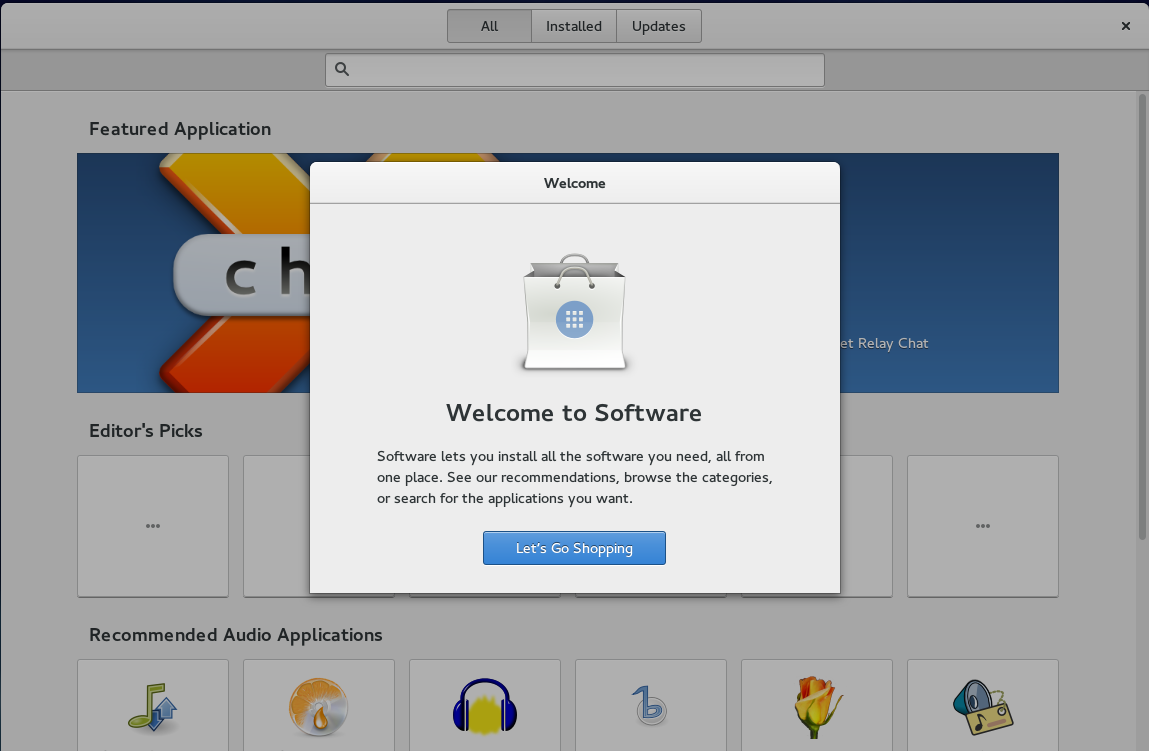
\includegraphics[keepaspectratio,width=\textwidth]{Gnome_software_welcome-cropped.png}
\end{figure}
The cornerstone of the Fedora Workstation is the Software installer, which lets you find all kinds of applications quickly and easily. The improvements to the Software installer in Fedora 21 provide a responsive and fast user experience. In addition, Fedora packagers have worked with developers around the world to greatly improve the number of featured applications.

\section{\textcolor{FedoraBlue}{Improvements to the terminal application}}

We want developers to have a great experience, so a strong Terminal application is absolutely important. We've integrated a set of additional features in the Terminal, such as:
\begin{itemize}
  \item Support for transparent backgrounds
  \item Automatic title updates to help you identify different terminals
  \item A simple toggle for disabling shortcuts in the Terminal
  \item Search for Terminals by name in the GNOME desktop overview
\end{itemize}

\section{\textcolor{FedoraBlue}{Experimental Wayland support}}
Wayland is a new and exciting display server technology that will power Linux desktops of the future. With Fedora Workstation 21 you can visit the future now, and see how well your applications work with Wayland. You can also experiment with making your applications take advantage of Wayland's new capabilities. Much of the core Wayland development comes from Fedora Workstation contributors, so this is your chance to try out Wayland straight from the source.



\section{\textcolor{FedoraBlue}{DevAssistant}}
\begin{figure}[h]
  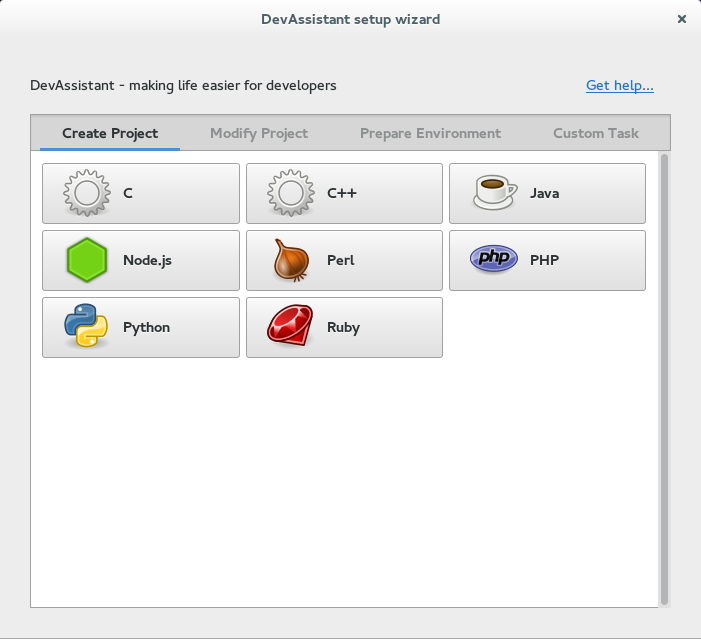
\includegraphics[keepaspectratio,width=\textwidth]{Fedora_devassistant-cropped.png}
\end{figure}
We recognize developers need an easy and straightforward way to set up many different programming environments. In Fedora Workstation, we offer the DevAssistant developer helper, which takes care of this setup for a large number of language runtimes and IDEs.

\section{\textcolor{FedoraBlue}{Ease of installation}}
\begin{figure}[h]
  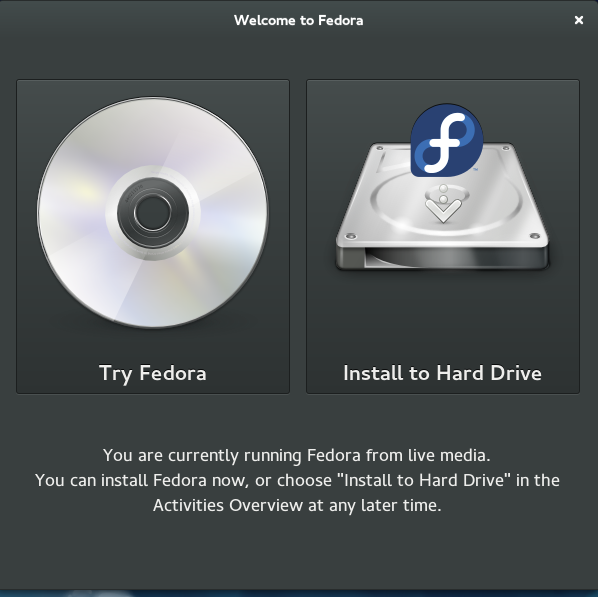
\includegraphics[keepaspectratio,width=\textwidth]{Workstation-anaconda-0-cropped.png}
\end{figure}
We want the installation of the Fedora Workstation to be as straightforward and simple as possible. In Fedora Workstation we've distilled this process down to selecting the layout of your physical media, and then pressing ``Install.'' (In fact, you can even let the installer choose the disk layout for you.) And because the future of installations is not optical disks, we ship with an easy to use tool to help you create bootable USB sticks -- just download a new Live image, right-click, and write to USB.

\section{\textcolor{FedoraBlue}{Web service integration}}
We recognize you have work to do, and you want to use the tools that let you get it done. That's why we're working to make all your applications in Fedora Workstation look and feel the same. With the ability to run HTML5 web services in a chromeless window, we aim to make your apps feel like a natural extension to your desktop. More integration upgrades are coming in future Fedora Workstation releases.

\section{\textcolor{FedoraBlue}{Support for high resolution displays (HiDPI)}}
Technology never stands still, and as a software developer you are used to using the best technology available. So we've spent a lot of time and effort on supporting the new generation of HiDPI displays found on new hardware like many new ultrabook models, or the Apple Retina display. That's probably why Fedora has been called the best of HiDPI.

\section{\textcolor{FedoraBlue}{Exciting roadmap}}
This Fedora Workstation release is not the end. It's the beginning of a new era for Fedora on the desktop. We have a roadmap lined up to bring a range of exciting new technologies to the Linux desktop:
\begin{itemize}
  \item Containers
  \item Smarter virtual machines
  \item Better development tools
  \item Improved toolkit integration
  \item More web integration
  \item \ldots and much more
\end{itemize}

So if you want to be part of the future of the Linux desktop, get on board now!
\newpage

\begin{center}
  {\color{FedoraBlue}
  \LARGE{Fedora Project\vspace{1cm}}
  \Large{\href{http://fedoraproject.org}{http://fedoraproject.org}}
}
\end{center}

\section{\textcolor{FedoraBlue}{Getting Support}}
\subsection{Fedora project wiki and mailing lists}
\href{https://fedoraproject.org/wiki/Communicate}{https://fedoraproject.org/wiki/Communicate}

\subsection{Official Documentation}
\href{http://docs.fedoraproject.org}{http://docs.fedoraproject.org}

\subsection{IRC Channel}
\href{http://webchat.freenode.net/?channels=#fedora}{\#fedora @ irc.freenode.net}

\subsection{Community forums}
\href{http://ask.fedoraproject.org}{http://ask.fedoraproject.org}
\href{http://fedoraforum.org}{http://fedoraforum.org}


\section{\textcolor{FedoraBlue}{Looking to join the Fedora community?}}
Are you interested in contributing to Fedora? There are many ways you can become active in the project.  Whether you are a People Person, Designer, OS Developer, Packager or Administrator - we have a place for you. Just head to the following page and get started today!

\begin{center}\href{http://join.fedoraproject.org}{http://join.fedoraproject.org}\end{center}


\end{document}
